\documentclass[12pt,letterpaper]{article}
\usepackage[T1]{fontenc}
\usepackage[utf8]{inputenc}
\usepackage{newtxtext}
\usepackage{newtxmath}
\usepackage[margin=1in]{geometry}
\usepackage{setspace}
\usepackage{parskip}
\usepackage{graphicx}
\usepackage{float}
\usepackage[hidelinks]{hyperref}
\usepackage{xcolor}
\usepackage{enumitem}
\usepackage{subcaption}

\setlength{\parindent}{0pt}
\setlength{\parskip}{0.6em}
\onehalfspacing

\definecolor{gcgreen}{HTML}{22B86A}
\newcommand{\GC}{\textcolor{gcgreen}{GreenCart}}

\title{\GC: IDH 3350 Semester Reflection}
\author{Tuan Khang Phan\\IDH 3350: Natural Science\\University of South Florida}
\date{Spring 2025}

\begin{document}
\maketitle

\section*{Quick Product Preview}

\begin{figure}[H]
  \centering
  \begin{subfigure}[t]{0.48\linewidth}
    \centering
    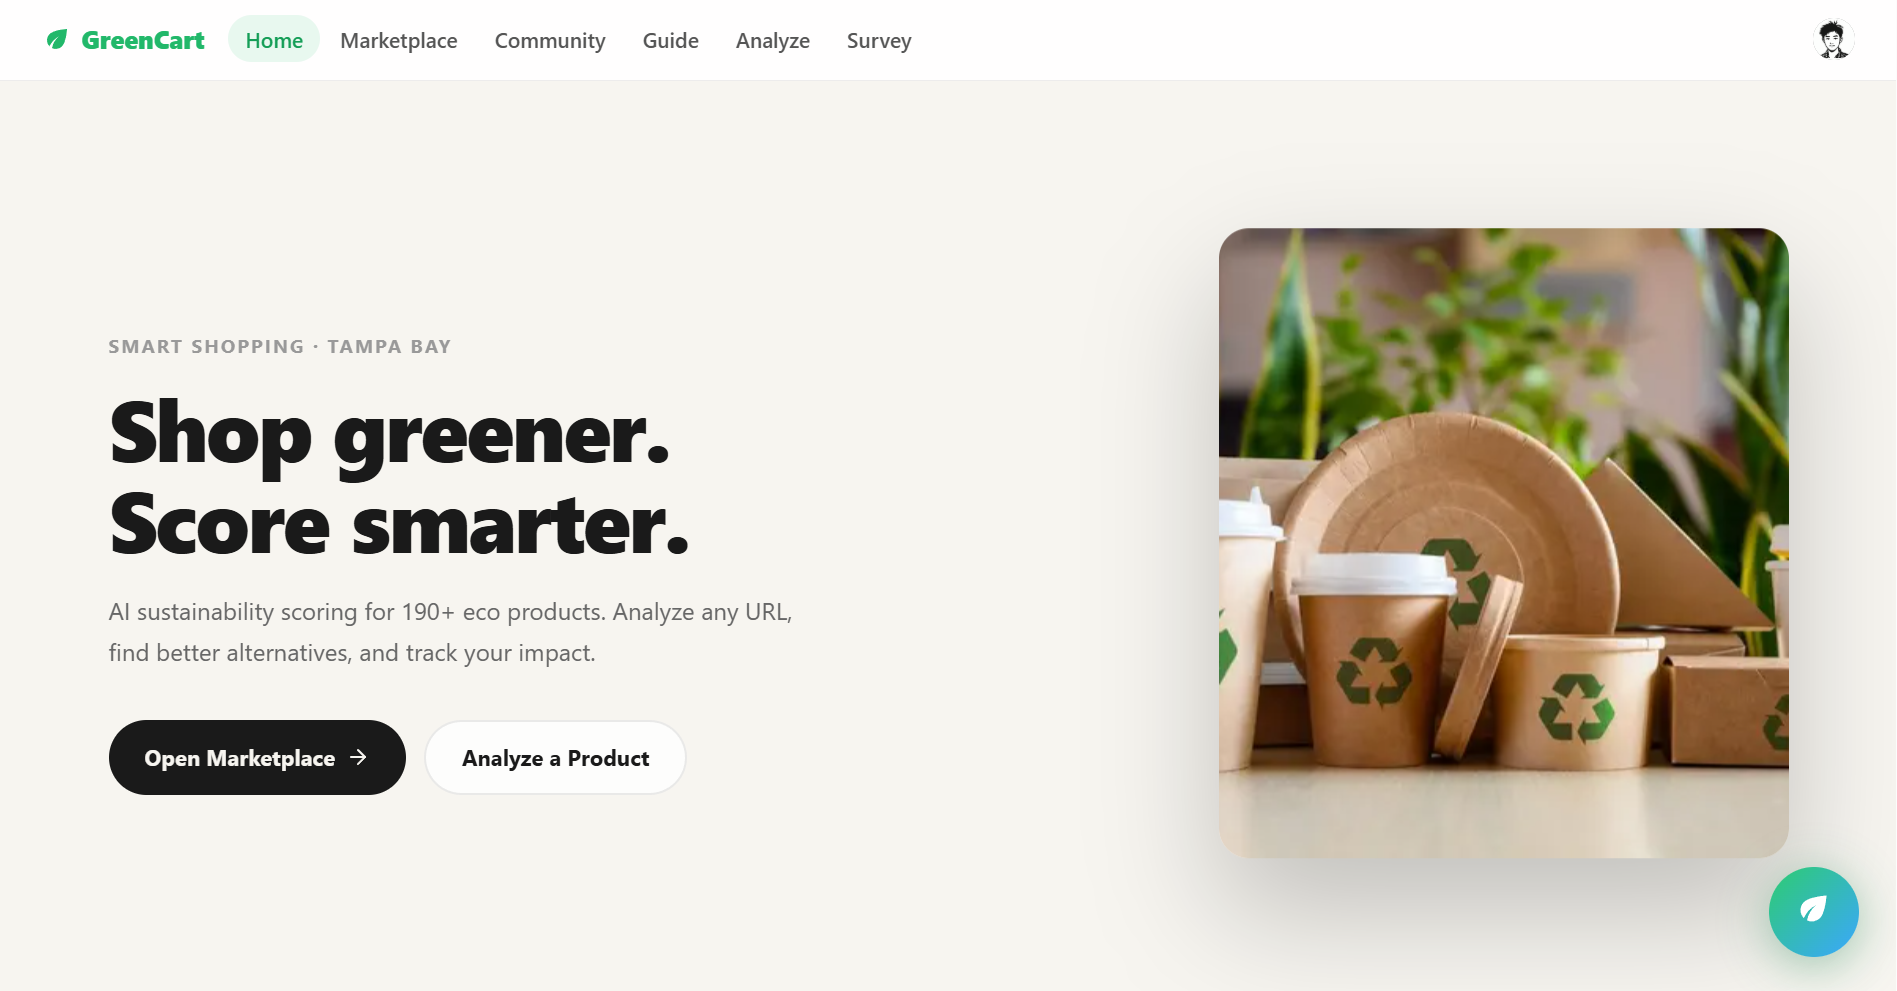
\includegraphics[width=\linewidth]{public/reflection/landing_page.png}
    \caption{Landing page of \GC.}
  \end{subfigure}
  \hfill
  \begin{subfigure}[t]{0.48\linewidth}
    \centering
    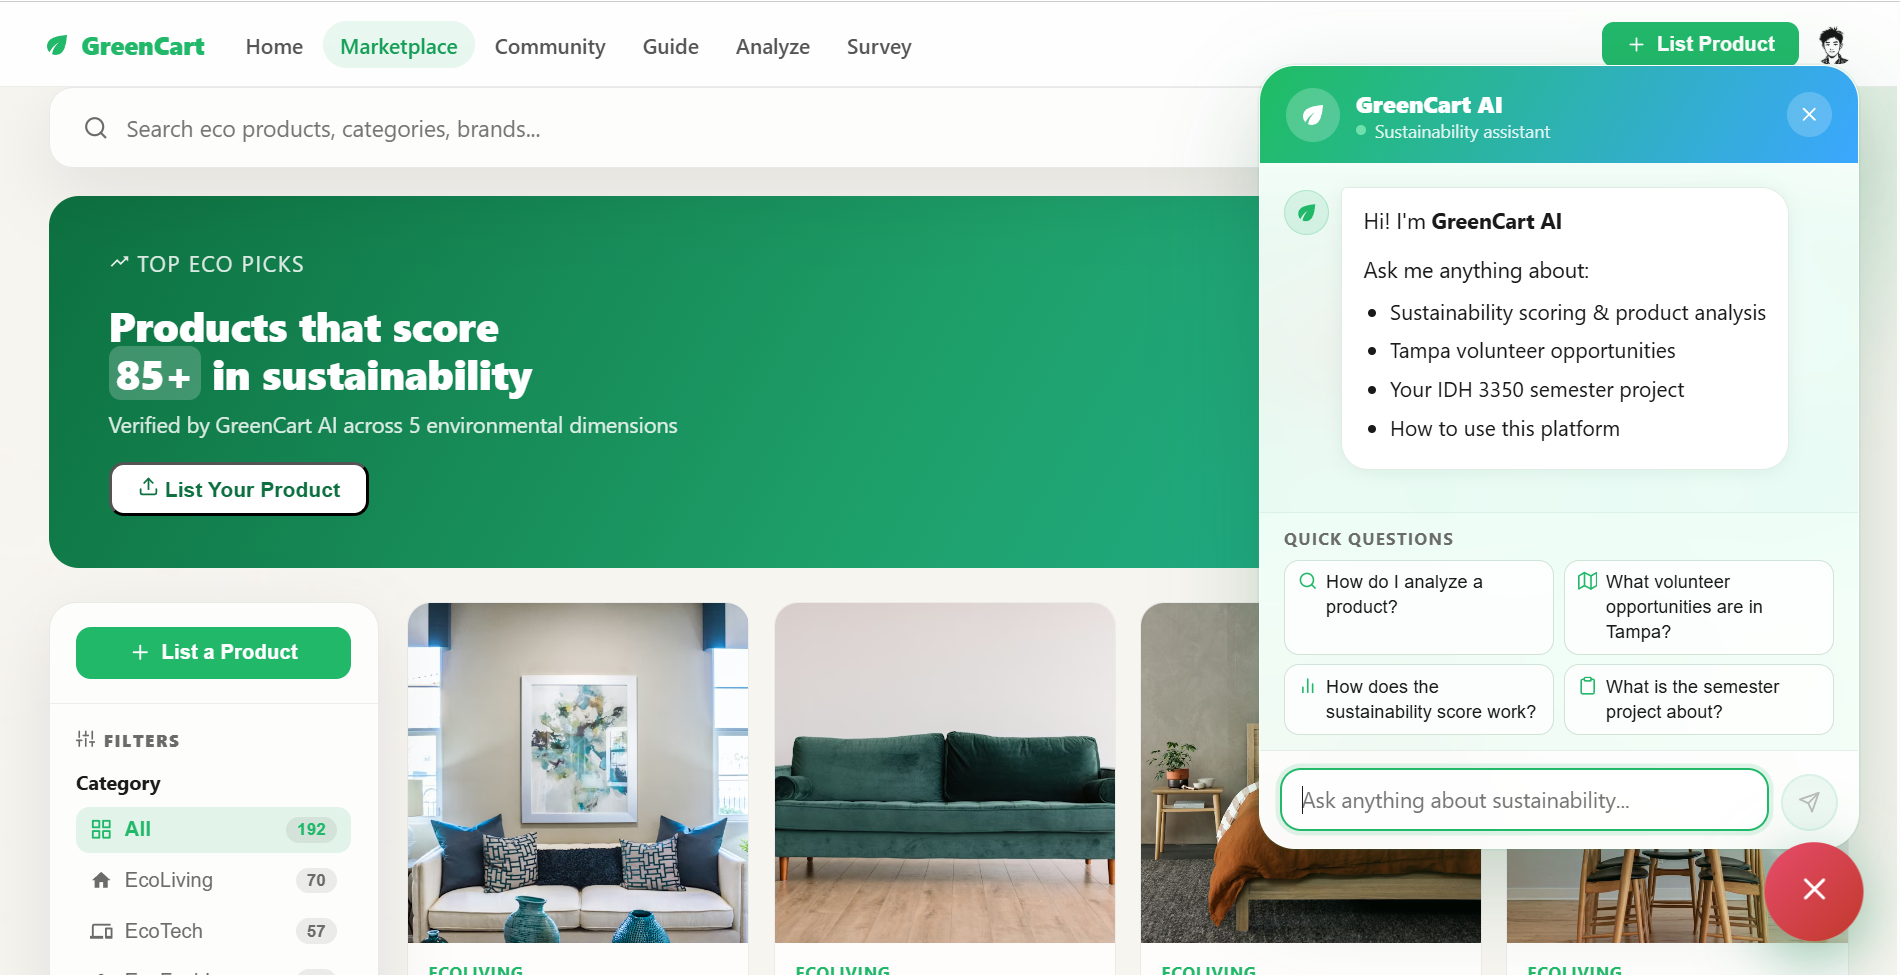
\includegraphics[width=\linewidth]{public/reflection/market_place.png}
    \caption{Marketplace view with curated eco products and filters.}
  \end{subfigure}
\end{figure}

The live platform is available at \href{https://green-space-three.vercel.app/}{green-space-three.vercel.app}, and a short video where I interviewed a few of my friends about their experience using the product can be found here: \textbf{\href{https://drive.google.com/drive/folders/1jYzF_xljhA-GoD0fElZIVsh9Vt4rkbEL}{Friends Interview Video (Google Drive)}}.

\section*{Reflection}

When I signed up for IDH 3350, I thought of the environment mostly as something that scientists study from far away. Forests, oceans, the atmosphere, ecosystems I had read about but never really felt responsible for. Over the semester, that picture slowly changed. The class kept returning to a simple but unsettling idea, which is that the environment is not somewhere out there. It is the room I sleep in, the food I pick up on the way to class, the electricity that keeps my laptop alive, and the water I drink without thinking. The more I sat with that idea, the more I wanted my semester project to do something real, something that touched my own community instead of staying in a notebook.

That is how \GC started. I wanted to build a small platform that helps students and local community members in Tampa Bay make more sustainable choices in their everyday life. Not a lecture, not a guilt trip, just a tool that quietly makes the greener option a little easier to see and a little easier to pick. I am a computer science student, so coding was the skill I had. But the project stopped being about code very quickly. It became about behavior, trust, and the quiet distance between what people believe and what they actually do at the checkout page.

In class we talked a lot about the attitude and behavior gap, the fact that most people already say they care about the planet but still reach for the cheaper, faster, less sustainable option when they are tired or busy. I saw this gap clearly in my own life. I would watch a documentary, feel moved, and then twenty minutes later add something to a cart without a second thought. I realized my own intentions were not enough, and that most people around me were living in the same quiet contradiction. \GC was my attempt to build a small bridge across that gap, so that the sustainable choice does not require extra research or extra guilt.

The product itself grew feature by feature over the semester. A marketplace with curated eco products. An AI powered analysis tool that reads a product link and gives an honest sustainability score across different environmental dimensions. A community page where people can share local volunteer opportunities and learn from each other. A survey section that asks students about their consumer habits, partly to collect data and partly to make them pause. A built in assistant that answers sustainability questions in plain language. Each of these pieces came from something we discussed in class, whether it was lifecycle thinking, environmental justice, collective action, or simple ecological literacy.

Doing interviews with my friends about the product turned out to be one of the most meaningful parts of the semester. I had expected polite feedback. What I got instead was honest conversation about how overwhelming sustainability can feel, how expensive some eco products seem, and how confused people are about what actually makes a difference. A few of them told me the AI analysis helped them understand why one item was better than another, which was the first time they felt like their choice was informed rather than lucky. Listening to them, I understood that the biggest environmental problem might not be a lack of care. It might be a lack of clarity. People are tired, and the planet is paying for that tiredness.

Working on this project also changed how I read the science we covered in class. Carbon footprints, biodiversity loss, water systems, and climate modeling used to feel like distant topics for someone else to solve. After a full semester of thinking about products, shipping, packaging, and local habits, those same topics felt personal. I started noticing things that used to be invisible to me, like how much packaging a single delivery creates, how much food the campus dining hall throws out at closing, and how often I drive when I could walk. These are tiny observations, but they are the kind of observations that only show up once you have decided to pay attention.

On the technical side, I will admit there were long nights when nothing worked and I wanted to quit. Databases broke, the AI gave strange answers, and deployments failed right before I wanted to show a friend. But each of those small failures taught me that building something for the environment is not a single heroic act. It is a quiet, repetitive practice of fixing, listening, and trying again. That is also how sustainability works in the real world. It is not a single lifestyle overhaul. It is a thousand small corrections, made consistently, by people who have decided that their community is worth the effort.

The class also pushed me to think beyond the individual. Personal choices matter, but systems matter more. A single student who recycles cannot undo a supply chain that is built around waste. That is why the community layer of \GC was important to me. Sharing volunteer opportunities, connecting students with local organizations, and making sustainability a social experience felt closer to the kind of collective action we read about. Change at scale tends to happen when people see others doing the same thing, and I wanted the platform to make that visibility possible, even in a small way.

Emotionally, this project was heavier than I expected. Climate anxiety is real, and there were weeks when reading the news made me wonder whether anything I built could possibly matter. What pulled me through was a sentence from one of our class discussions, the idea that engaged citizens live their lives today to create the futures they want to become a reality. I cannot fix the climate crisis with a web app. But I can build something useful for the people around me, and I can keep building. That feels like a future worth working toward.

Looking back, \GC made me a more grounded person. I am more careful with what I buy, more curious about where things come from, and more patient with friends who are still figuring it out, because I am still figuring it out too. I plan to keep developing the platform after the class ends. I want to expand the local community features, improve the analytics behind the survey, and eventually partner with student organizations on campus so that the tool grows beyond me. I also want to keep making short interviews and conversations a part of the project, because the most honest insights I gathered this semester came from simply asking people what they actually do.

If this class taught me one thing, it is that the environment is not a topic. It is a relationship. It is the slow, ongoing conversation between a person and the place they live in. \GC is my contribution to that conversation right now, and I am grateful the class gave me a reason to start it. I will keep going.

\section*{Links}
\begin{itemize}[leftmargin=1.2em]
  \item Platform: \href{https://green-space-three.vercel.app/}{green-space-three.vercel.app}
  \item Friends interview video: \textbf{\href{https://drive.google.com/drive/folders/1jYzF_xljhA-GoD0fElZIVsh9Vt4rkbEL}{Google Drive folder}}
  \item Research blog: \href{https://env-blog.vercel.app/}{env-blog.vercel.app}
\end{itemize}

\end{document}
